\documentclass[../thesis.tex]{subfiles}
\begin{document}

\chapter{Simulation Model}
\label{chp:model}

Within this part the creation process of the simulation model will be explained in greater detail. At first the geometry modelling, meshing and solver setup will be explained. Later on, the mesh dependency study and the model validation are explained.

\section{Model Setup}
\label{sec:mod_setup}
In this section the steps needed to create the model within \texttt{ANSYS FLUENT} are explained.

\subsection{Geometry Creation}
The first step of the model creation in \texttt{ANSYS FLUENT} is the modelling of the system geometry. This geometry can either be created using the tools \texttt{ANSYS FLUENT} provides or be imported from an already existing CAD model. Within this work the geometry is created using \texttt{ANSYS DesignModeler}. In \autoref{fig:ansys_geometry} a sketch of the designed model is shown and the used dimensions are listed in \autoref{tab:ansys_design}.
\begin{figure}[htbp]
	\centering
	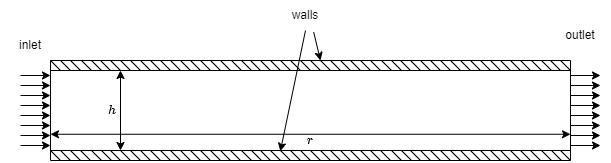
\includegraphics[width=\textwidth]{geometry}
	\caption{Sketch of the model geometry including outer dimensions}
	\label{fig:ansys_geometry}
\end{figure}
\begin{table} [htb]
	\centering
	\caption{Used values for geometry dimensions}
	\begin{tabular}{ ccc }
		\hline
		variable & value & unit \\
		\hline
		$r$ & 30.0 & mm \\
		$h$ & 0.2...0.6 & mm \\
		\hline
		\label{tab:ansys_design}
	\end{tabular}
\end{table}

$h$ represents the height of the Hele-Shaw cell and $r$ is the radius of the cell. A value of 30mm is chosen here. For the used settings the front does not travel the whole 50mm, so this simplification does not effect the results as can be seen in later sections.

\subsection{Meshing}
In this section the mesh creation process is explained in greater detail. An example of the generated mesh can be seen in \autoref{fig:ansys_meshing}.
\begin{figure}[htb]
	\centering
	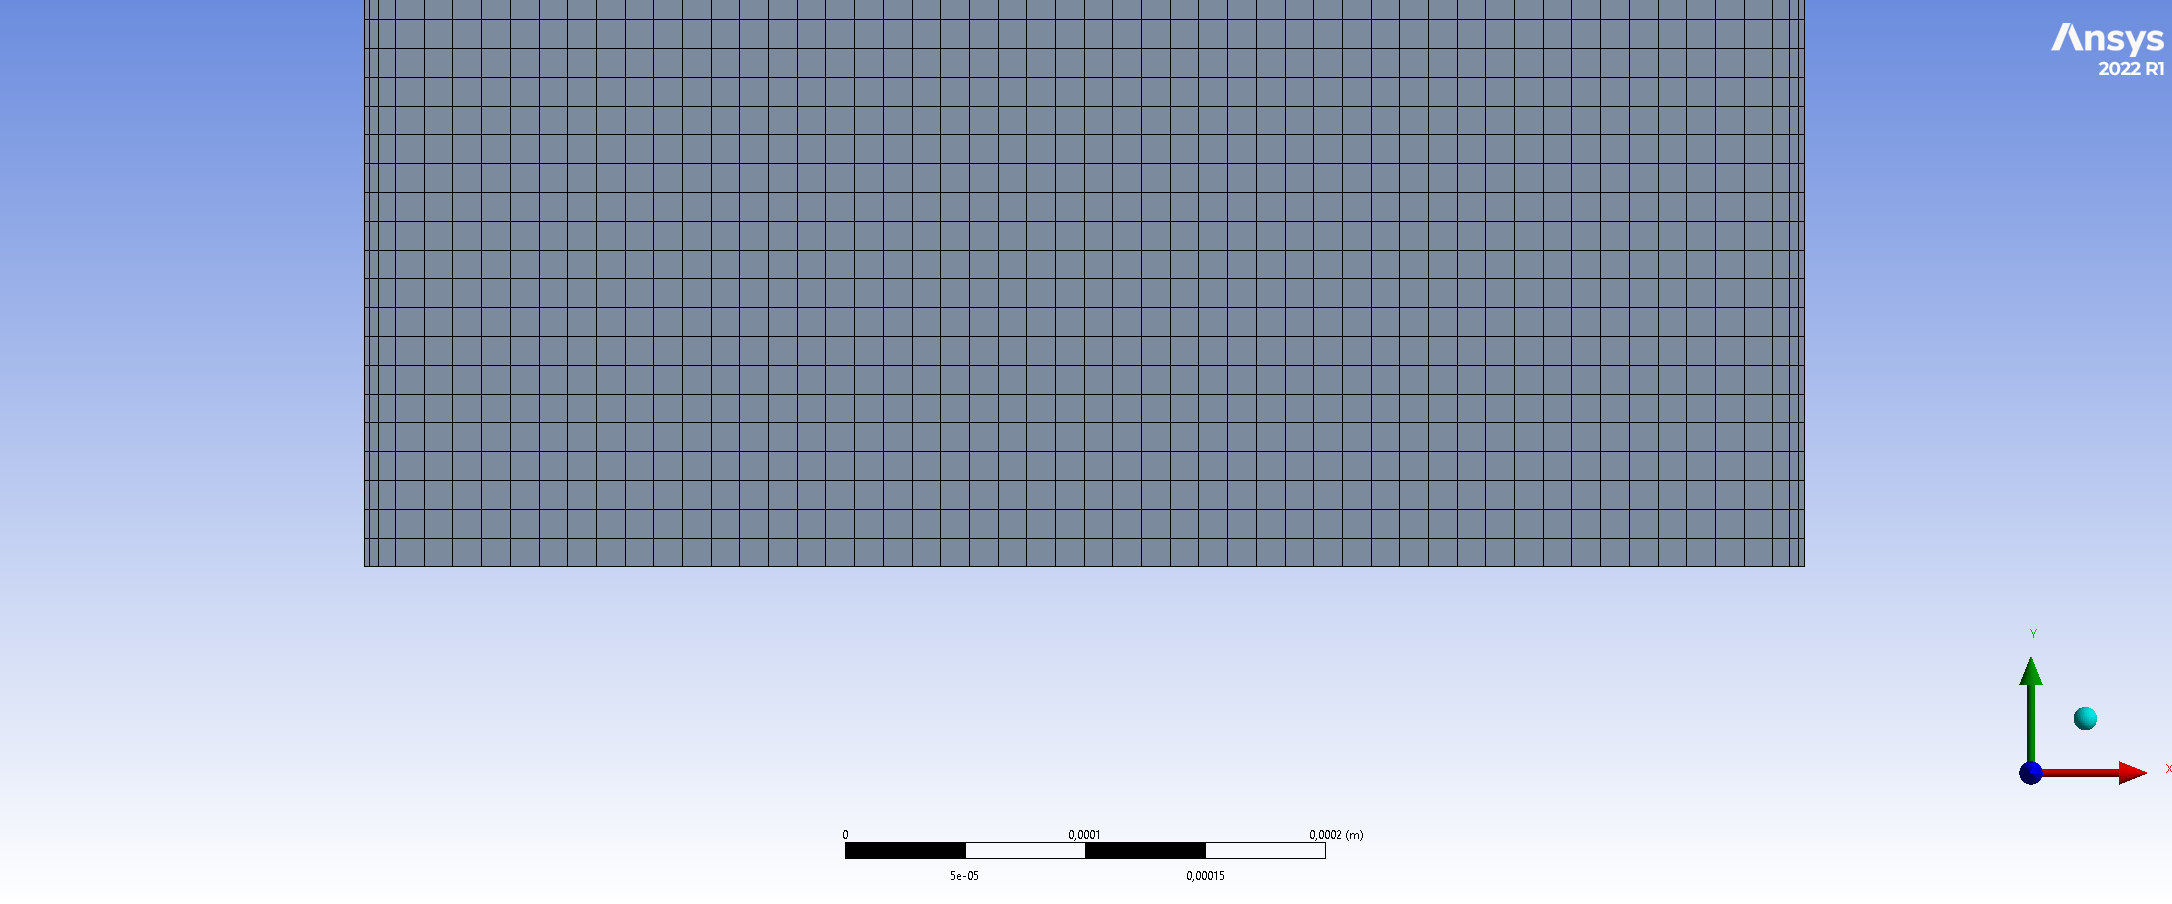
\includegraphics[scale=0.25]{Mesh}
	\caption{Ansys Meshing example}
	\label{fig:ansys_meshing}
\end{figure}
The figure shows the reactor's inlet section. The goal in meshing this geometry is to create a rectangular grid out of squares or rectangles. Near the walls, that begin on the left and right side of the inlet, the mesh resolution is increased using two inflation layers. That is done to resolve the boundary layer of the flow near the walls. These finer resolutions near the wall are needed, because near the wall the flows velocity does show large gradients \cite{versteeg2007introduction}. Having a mesh consisting mostly out of squares and rectangles is advantageous because the algorithm only stores the values at the cell's centre as mentioned in \autoref{sec:QUICK} and having a mesh that can be seen as a 2 dimensional array helps with post-processing. The detailed results and their analysis are discussed in \autoref{sec: model res}.

\subsection{Solver Settings}
\label{sec: setup}

To setup the model at first a few general configuration steps need to done. The Settings that need to be applied are listed in \autoref{tab:ansys_setup_general}.

\begin{table} [htb]
	\centering
	\caption{General model settings}
	\begin{tabular}{ ccc }
		\hline
		Section & Setting & value \\
		\hline
		Solver & Type & Pressure-Based \\
		Solver & Velocity Formulation & Absolute  \\
		Solver & Time &  Transient  \\
		Solver & 2D Space & Axisymmetric \\
		\hline
		\label{tab:ansys_setup_general}
	\end{tabular}
\end{table}
The type of solver chosen is a Pressure-Based that also is the default value. The velocity formulation is set to \texttt{Absolute} because the input velocity is set to an absolute value. The \texttt{Time} setting is set to \texttt{Transient} because the flow modelled is not stationary and the interest is in results during the whole models simulation run. The \texttt{2D Space} settings has a value of \texttt{Axisymmetric} due to the axisymmetric nature of the geometry. The Viscous model is set to \texttt{Laminar} because laminar flow conditions are used. Due to a reaction being part of the model the energy variable needs to be set to \texttt{On}.

After the correct models are turned on and parametrized the species taking part within the model are defined. Within this case 4 fluids are needed. The example configuration of one of the fluids taking part within the reaction is shown in \autoref{tab:ansys_setup_materials}. The table shows the configuration of one of the reactants.
\begin{table} [htb]
	\centering
	\caption{Fluid mixture settings}
	\begin{tabular}{ ccc }
		\hline
		variable & value & unit \\
		\hline
		\\[-1em]
		$\rho$ & 1000 & $\frac{\text{kg}}{\text{m³}}$ \\
		\\[-1em]
		$\nu$ & 1.0e-6...1.2e-6 & $\frac{\text{m²}}{s}$ \\
		\\[-1em]
		$D$ & 1.00e-10...8.22e-10 & $\frac{\text{m²}}{s}$\\
		\\[-1em]
		\hline
		\label{tab:ansys_setup_materials}
	\end{tabular}
\end{table}
All other values, namely enthalpies and other thermodynamic properties are the same for all the fluids and equal to the values of water. Since 3 fluids take part in the reaction and 4 fluids are needed to setup the model the yet missing fluid is water. It is needed to be able to set a molar concentration at the inlet. With the mixture settings the reaction parameters are set. The parameters set for the reaction are stated in \autoref{tab:ansys_setup_rection}.
\begin{table} [htb]
	\centering
	\caption{reaction settings}
	\begin{tabular}{ ccc }
		\hline
		variable & value & unit \\
		\hline
		Reaction Type & Volumetric & - \\
		Stoich. Coefficient fluid\_a & 1 & - \\
		Stoich. Coefficient fluid\_b & 1 & - \\
		Stoich. Coefficient fluid\_c & 1 & - \\
		Rate Exponent fluid\_a & 1 & - \\
		Rate Exponent fluid\_b & 1 & - \\
		Rate Exponent fluid\_c & 0 & - \\
		\\[-1em]
		Pre-Exponential Factor & 1e15 & $\frac{\text{l}^2}{\text{s} \cdot \text{mol}}$ \\
		\\[-1em]
		Activation Energy & 1e4 & $\frac{\text{J}}{\text{mol}}$ \\
		\\[-1em]
		\hline
		\label{tab:ansys_setup_rection}
	\end{tabular}
\end{table}
To achieve a nearly instant reaction when molecules of the two species A and B meet the rate constant which is also known as Pre-Exponential Factor (see \autoref{eqn:reaction}) is set to $1 \cdot 10^{15} \left[ \frac{\text{l}^2}{\text{s} \cdot \text{mol}} \right]$. The Activation Energy is set to a value of $ 1 \cdot 10^{4} \left[\frac{\text{J}}{\text{mol}}\right]$. With that value, the given temperature of $300 [\text{K}]$ is high enough to let the reaction happen.
After the reaction is setup correctly the boundary conditions are being set. Boundary conditions need to be set for the inlet, outlet and the walls. All information needed to configure the boundary conditions are visible in \autoref{tab:ansys_setup_boundary}. As part of the boundary conditions the flow domain has to be initialized with values to start the simulation from. To achieve the same conditions as within the experimental setup the reactor is filled with species $B$ with a concentration of $0\text{.}03 \left[\frac{\text{mol}}{\text{l}}\right]$. Mole fractions $x_i$ are required as inputs for the inlet, so they have to be calculated from the given concentration using \autoref{eqn:molefrac}.
\begin{equation}
	\label{eqn:molefrac}
	\begin{split}
		x_{fluid\_a} & =\dfrac{\dot{n_{fluid\_a}}}{\dot{n_{fluid\_a}} + \dot{n_{water}}} \\[0.5em]
		& = \dfrac{c_{fluid\_a} \cdot Q}{c_{fluid\_a} \cdot Q + c_{water} \cdot Q} \\[0.5em]
		& = \dfrac{c_{fluid\_a}}{c_{fluid\_a} + c_{water}}
	\end{split}
\end{equation}
The initialization of the domain requires mass fractions $\varphi_i$ so they need to be calculated as well using \autoref{eqn:massfrac}. In addition to the mass fraction the internal domain is initialized with a pressure of $20$[Pa] and a temperature of $300$[K]. To get a homogenous velocity profile at the inlet normal to the boundary, the specification method is set to \texttt{Magnitude, Normal to Boundary}.
\begin{equation}
	\label{eqn:massfrac}
	\begin{split}
		\varphi_{fluid\_b} & = \dfrac{n_{fluid\_b} \cdot M_{fluid\_b}}{n_{fluid\_b} \cdot M_{fluid\_b} + n_{water} \cdot M_{water}} \\[1em]
		& = \dfrac{c_{fluid\_b} \cdot M_{fluid\_b}}{c_{fluid\_b} \cdot M_{fluid\_b} + c_{water} \cdot M_{water}} \\
	\end{split}
\end{equation}

\begin{table} [htb]
	\centering
	\caption{Models boundary conditions}
	\begin{tabular}{ cccc }
		\hline
		place & variable & value & unit \\
		\hline
		inlet & Type & velocity-inlet & - \\
		inlet & Velocity Specification Method & Magnitude, Normal to Boundary & - \\
		\\[-1em]
		inlet & Velocity Magnitude & 8.33e-5...4.21e-3 & $\frac{\text{m}}{\text{s}}$ \\
		\\[-1em]
		inlet & Temperature & 300 & K \\
		inlet & $x_{fluid\_a}$ & 5.4e-4 & - \\
		outlet & Type & pressure-outlet & - \\
		outlet & Gauge Pressure & 20 & Pa \\
		outlet & Prevent Reverse Flow & yes & - \\
		wall & Type & wall & - \\
		wall & Shear Condition & No Slip & - \\
		\hline
		\label{tab:ansys_setup_boundary}
	\end{tabular}
\end{table}
In \autoref{tab:ansys_setup_molefrac} the properties of the species taking part in the reaction are shown. The molar masses for species $A$ and $B$ are the same and the product $C$ has a value that is twice as high as the one of the species $A$ or $B$. The molar masses are set that way to ensure the reaction $A+B \rightarrow C$ takes place with one mole of $A$ and $B$ do result in one mole of product $C$. The densities are set to 1000$ \left[\frac{\mathrm{kg}}{\mathrm{m}^3}\right] $ for all species.
\begin{table} [htb]
	\centering
	\caption{Mixture species properties}
	\begin{tabular}{ cccc }
		\hline
		variable & description & value & unit \\
		\hline
		\\[-1em]
		$M_{water}$ & Molar Mass water & 18 & $\frac{\mathrm{g}}{\mathrm{mol}}$ \\
		\\[-1em]
		$M_{fluid\_a}$ & Molar Mass $fluid\_a$ & 100 & $\frac{\mathrm{g}}{\mathrm{mol}}$ \\
		\\[-1em]
		$M_{fluid\_b}$ & Molar Mass $fluid\_b$ & 100 & $\frac{\mathrm{g}}{\mathrm{mol}}$ \\
		\\[-1em]
		$M_{fluid\_c}$ & Molar Mass $fluid\_c$ & 200 & $\frac{\mathrm{g}}{\mathrm{mol}}$ \\
		\\[-1em]
		$\rho_{water}$ & Density water & 1000 & $\frac{\mathrm{kg}}{\mathrm{m}^3}$ \\
		\\[-1em]
		$\rho_{fluid\_a}$ & Density $fluid\_a$ & 1000 & $\frac{\mathrm{kg}}{\mathrm{m}^3}$ \\
		\\[-1em]
		$\rho_{fluid\_b}$ & Density $fluid\_b$ & 1000 & $\frac{\mathrm{kg}}{\mathrm{m}^3}$ \\
		\\[-1em]
		$\rho_{fluid\_c}$ & Density $fluid\_c$ & 1000 & $\frac{\mathrm{kg}}{\mathrm{m}^3}$ \\
		\\[-1em]
		$c_{fluid\_a}$ & Concentration $fluid\_a$ & 0.03 & $\frac{\mathrm{mol}}{\mathrm{l}}$ \\
		\\[-1em]
		$c_{fluid\_b}$ & Concentration $fluid\_b$ & 0.03 & $\frac{\mathrm{mol}}{\mathrm{l}}$ \\
		\\[-1em]
		$x_{fluid\_a}$ & molar fraction $fluid\_a$ & 5.4e-4 & - \\
		\\[-1em]
		$x_{fluid\_b}$ & molar fraction $fluid\_b$ & 5.4e-4 & - \\
		\\[-1em]
		$\varphi_{fluid\_a}$ & mass fraction $fluid\_a$ & 3e-3 & - \\
		\\[-1em]
		$\varphi_{fluid\_b}$ & mass fraction $fluid\_b$ & 3e-3 & - \\
		\\[-1em]
		\hline
		\label{tab:ansys_setup_molefrac}
	\end{tabular}
\end{table}

The temperature is set to 300[K] at the inlet. The outlet is configured to be a pressure outlet without reverse flow to get physically valid results. At the walls the usual conditions applied to walls are set with no slip.

The next step performed is to setup the solution methods as shown in \autoref{tab:ansys_setup_sol_methods}. As the solving scheme the PISO algorithm is used, that is explained in \autoref{sec:sol_method}. For spatial discretization second order methods, as explained in \autoref{sec:QUICK}, are used. 
\begin{table} [htb]
	\centering
	\caption{Solution methods}
	\begin{tabular}{ ccc }
		\hline
		tab & setting & method \\
		\hline
		Pressure-Velocity Coupling & Scheme & PISO \\
		Spatial Discretization & Pressure & Second Order \\
		Spatial Discretization & Momentum & QUICK \\
		Spatial Discretization & $fluid\_a$ & Second Order Upwind \\
		Spatial Discretization & $fluid\_b$ & Second Order Upwind \\
		Spatial Discretization & $fluid\_c$ & Second Order Upwind \\
		Spatial Discretization & Energy & Second Order Upwind \\
		\hline		
		\label{tab:ansys_setup_sol_methods}
	\end{tabular}
\end{table}

As a last step in the model creation procedure the time discretization parameters need to be set. An adaptive method is chosen which is based on the CFL-Number $c$. The CFL-Number is another name for the Courant number. It is best practice to keep this number below or equal to 1 for stability reasons. This can be otherwise thought of as a limiting factor in a way that to rapid changes from one cell to the next one between time steps are inhibited.
  
In this model the Courant number is set to 1 and the initial time step size is set to the same value as the minimum time step. The time step size is updated after every calculation. The factor for time step changes are limited to 0.5 on the lower and 2 at the upper end. The time step algorithm decides for a time step change based on the Courant number. In most cases the time step used by the solver has a value close to the minimum time step size of values around 0.001 seconds. The minimum time step is set dependant on the inlet velocity. In addition to the model's time settings the interval the results are exported at need to be set.
\begin{table} [htb]
	\centering
	\caption{Time discretization parameters}
	\begin{tabular}{ ccc }
		\hline
		variable & value & unit \\
		\hline
		Type & Adaptive & - \\
		Method & CFL-Based & - \\
		Duration Specification Method & Total Time & -\\
		Total Time & 60...360 & s \\
		Courant Number & 1 & - \\
		Fixed Timsteps & 1 & - \\
		Initial Time Step Size & 1e-4...2.5e-3 & s \\
		Max Iteration/Time Step & 30 & - \\
		Time Step Size Update Interval & 1 & - \\
		Minimum Time Step Size & 1e-4...2.5e-3 & s \\
		Maximum Time Step Size & 0.5 & s \\
		Minimum Step Change Factor & 0.5 & - \\
		Maximum Step Change Factor & 2 & - \\		
		\hline
		\label{tab:ansys_setup_time}
	\end{tabular}
\end{table}

\section{Model Evolution}
\label{sec: mod_evol}

Here the steps taken to receive the final model for each case are explained.

\subsection{Mesh Dependency}
\label{sec: mesh_dep}

To achieve trustworthy results from a CFD-model the solution obtain should be not dependent of the grid element size. 
To do that for each case different meshes with different grid densities are created as shown in \autoref{tab: reactor meshes}.
\begin{table} [htb]
	\centering
	\caption{case meshes}
	\begin{tabular}{ ccc }
		\hline
		reactor height [mm] & element size [m] & mesh elements \\
		\hline
		0.2 & 6e-6 & 185000\\
		0.2 & 4e-6 & 405000\\
		0.2 & 2e-6 & 1560000\\
		0.4 & 12e-6 & 92500\\
		0.4 & 8e-6 & 202500\\
		0.4 & 4e-6 & 780000\\
		0.6 & 4e-6 & 1155154\\
		0.6 & 2e-6 & 4560304\\
		\hline		
		\label{tab: reactor meshes}
	\end{tabular}
\end{table}
Each case is run for the coarsest mesh and the results are inspected. The first indication for a fine enough mesh can be extracted from the Courant number field. An example of a right and wrong field is shown in \autoref{fig: good_courant}. If as within the example, the field shows values higher than 1 the next finer mesh is chosen and the simulation is run again. If that is not the case the grid is chosen for the case and the run is called successful.

\begin{figure}[htb]
	\centering
	\subfloat[\centering Wrong Courant number field for an example case]{{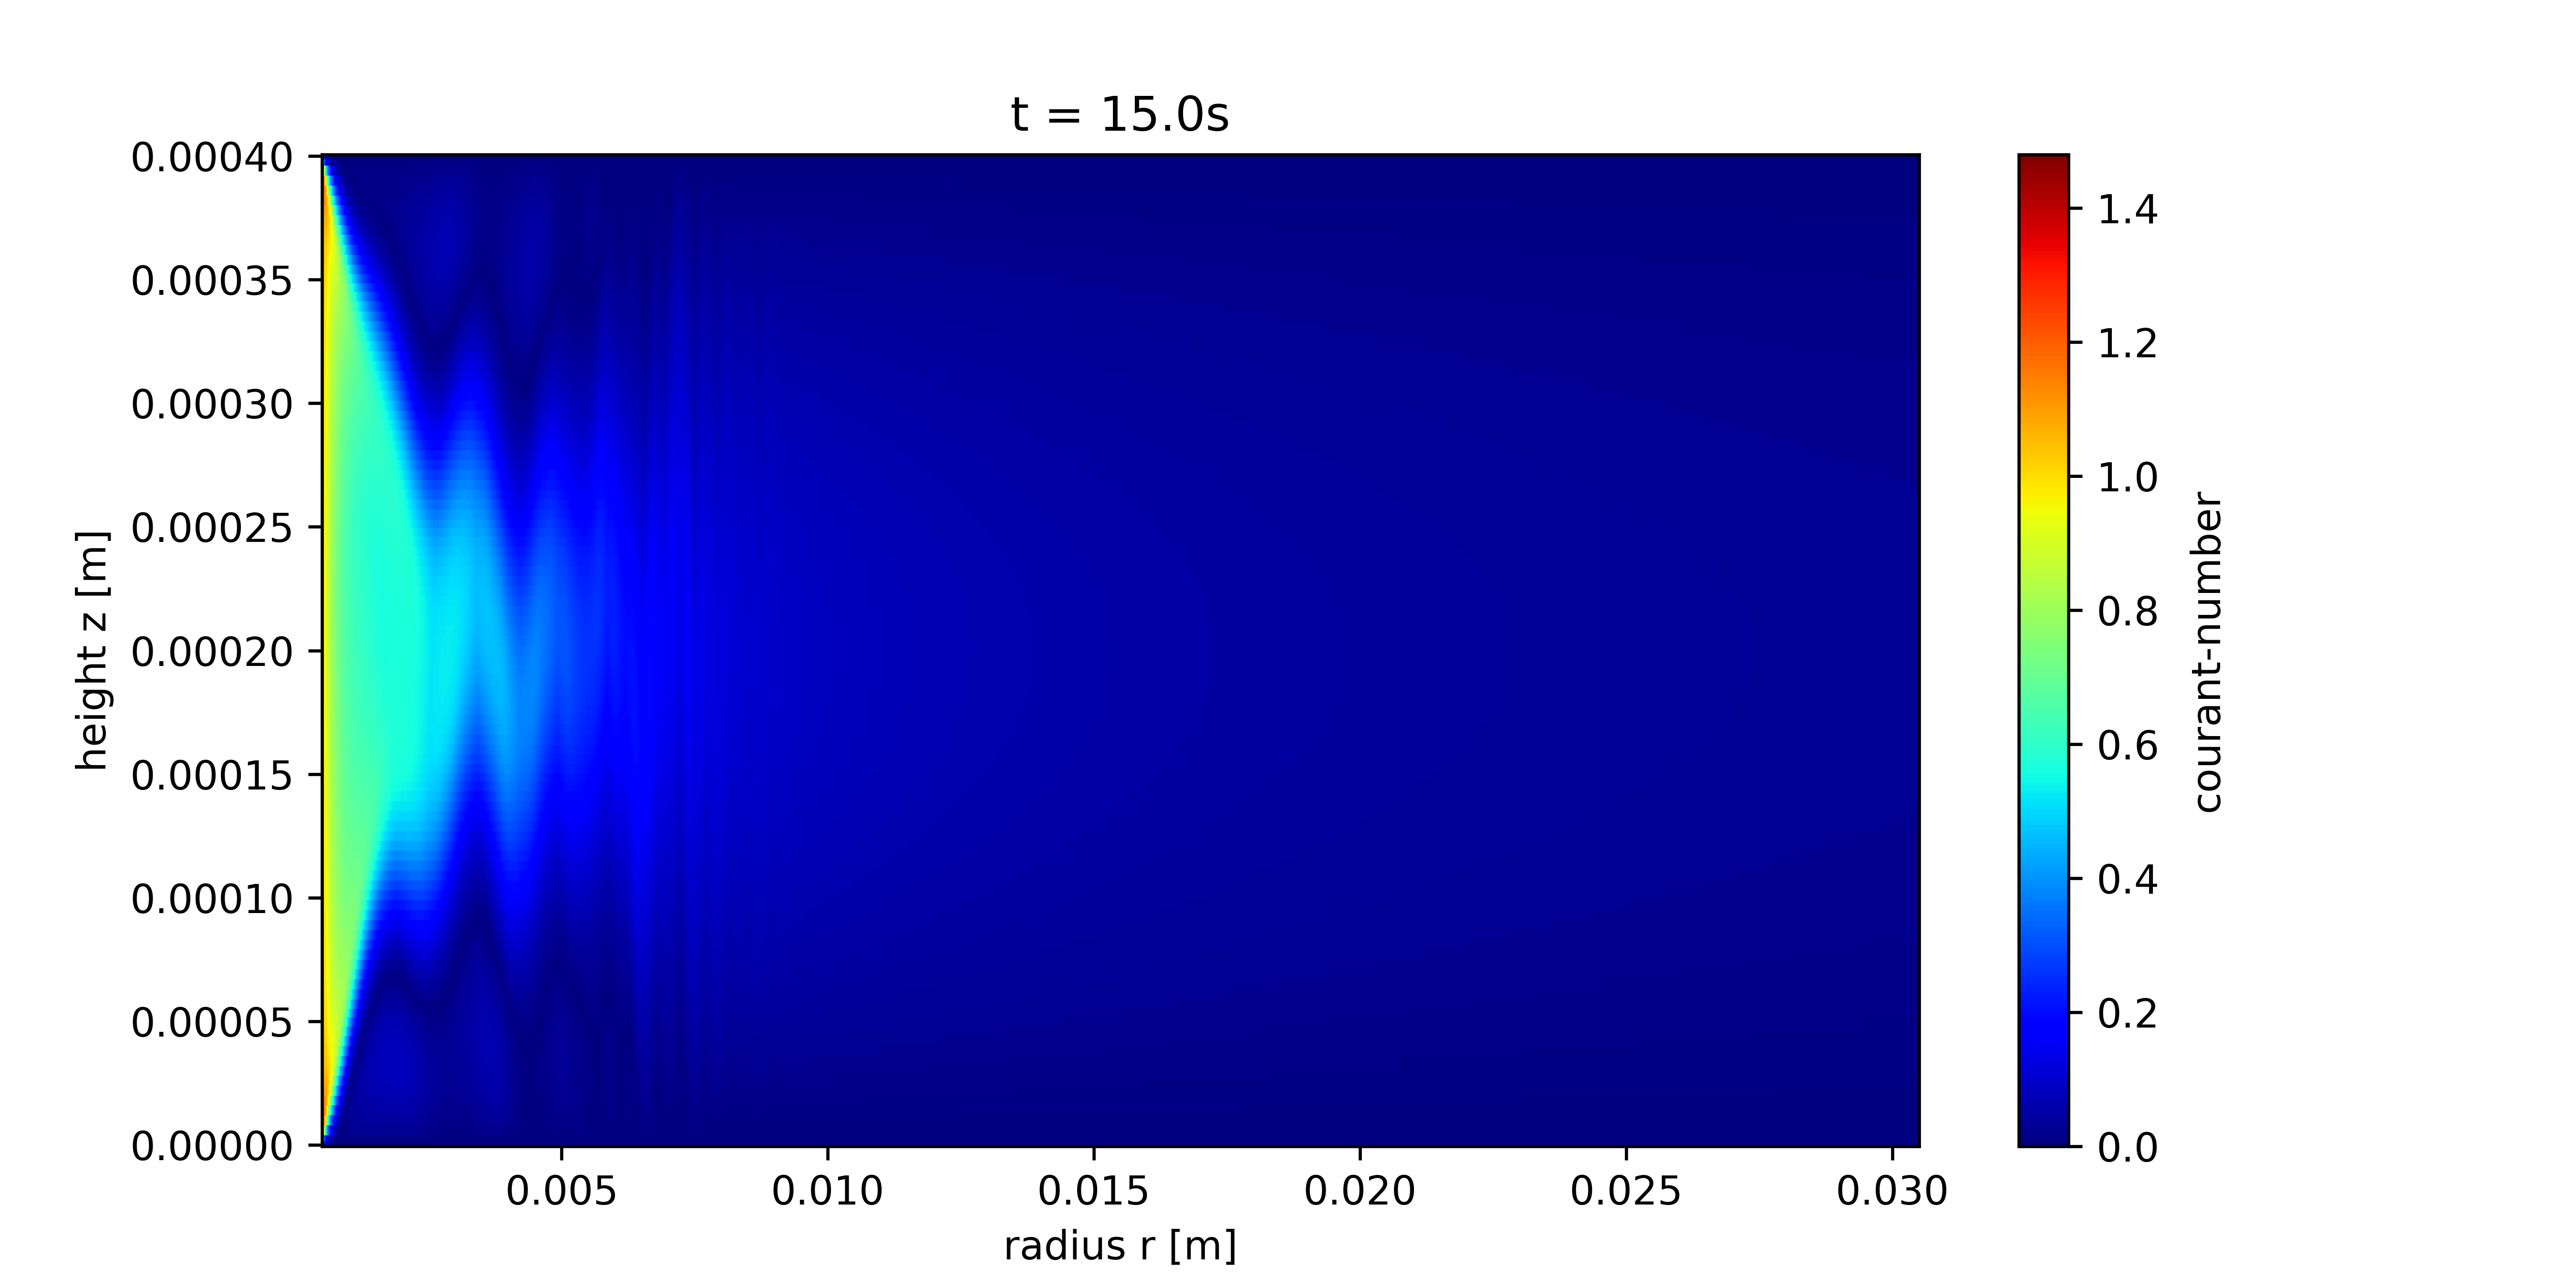
\includegraphics[scale=0.7]{bad_courant} }}
	\qquad
	\subfloat[\centering Right Courant number field for another example case]{{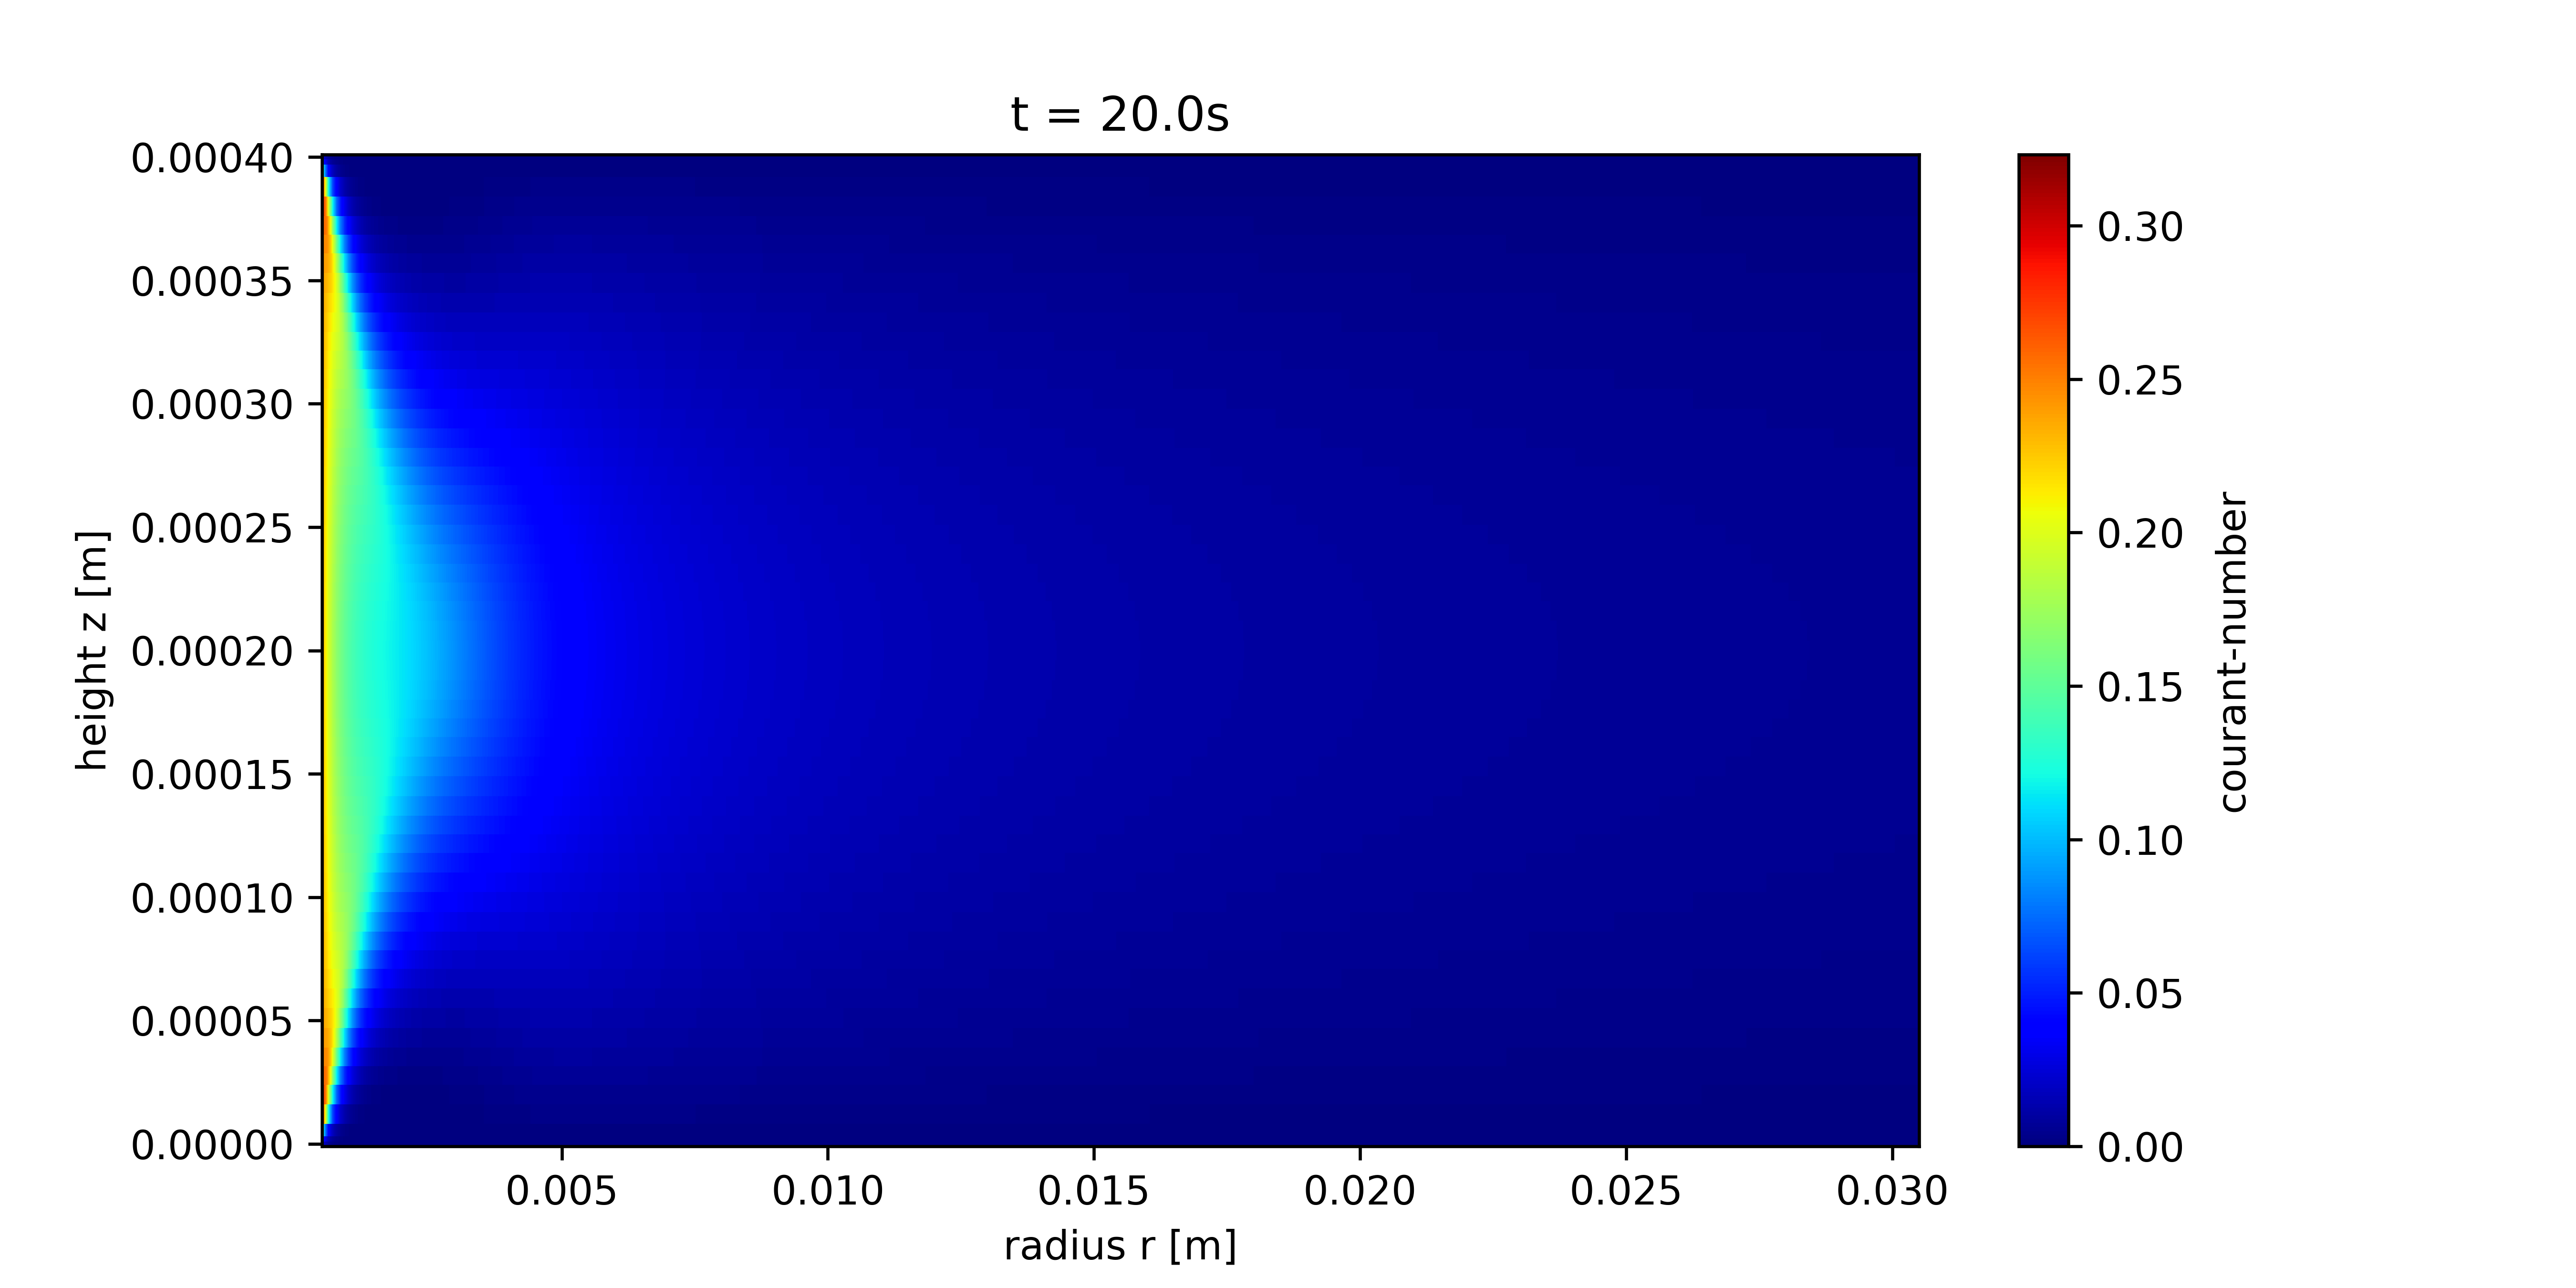
\includegraphics[scale=0.7]{good_courant} }}
	\caption{wrong and right example of Courant number field for mesh dependency study}
	\label{fig: good_courant}
\end{figure}
With this method a fine enough mesh for each case is chosen so that the results can be trusted.

\subsection{Cases Setup}

For the Peclet-Number 3 different values are chosen and for the Schmidt number 2 values are implemented. These values are in case of $Pe$ 500, 931 and 2050. The Peclet number values are set to close to values experimental data is available for. The Schmidt number $Sc$ has either a value of 2430 or 12000. The lower value is chosen to match existing experimental results and the higher one set to see a significant change compared to the lower one. The Schmidt number mostly influences the diffusion coefficient as the viscosity $\nu$ does not change a lot between the two chosen values. Having fixed the Schmidt number and the diffusion coefficient, the Peclet-Number mostly influences the input velocity. An overview of the performed cases and their input variable values can be seen in \autoref{tab: cases}. Besides the reactor height $h$, the Peclet-Number $Pe$ and other needed input variables, the simulation time and export time in seconds need to be set. The simulation time is the physical time that represents for how long the model should be simulated. The export time sets the time interval in seconds at which results are exported during the transient simulation. These results, that contain all the values for all variables of interest for each cell, are the basis for further analysis. Section \ref{sec: model res} explains how the results are further processed in more detail.
\begin{landscape}
	\begin{table}[htb]
		\centering
		\caption{simulation cases}
		\label{tab: cases}
		\small
		\begin{tabular}{cccccccccc}
			\textbf{h [m]} & \textbf{Pe} & \textbf{Sc} & \textbf{$\nu$ [m²/s]} & \textbf{$D$ [m²/s]} & \textbf{u [m/s]} & \textbf{$x_A$} & \textbf{$\varphi_B$} & \textbf{simulation time [s]} & \textbf{export time [s]} \\
			\hline
			2.00E-04            & 500         & 2430        & 1.00E-06               & 4.11E-10               & 1.03E-03              & 5.40E-04      & 3.00E-03        & 60                            & 0.5                       \\
			2.00E-04            & 500         & 12000       & 1.20E-06               & 1.00E-10               & 2.50E-04              & 5.40E-04      & 3.00E-03        & 60                            & 0.1                       \\
			2.00E-04            & 500         & 120000      & 1.20E-06               & 1.00E-11               & 2.50E-05              & 5.40E-04      & 3.00E-03        & 60                            & 0.1                       \\
			2.00E-04            & 931         & 2430        & 1.00E-06               & 4.11E-10               & 1.91E-03              & 5.40E-04      & 3.00E-03        & 60                            & 0.5                       \\
			2.00E-04            & 931         & 12000       & 1.20E-06               & 1.00E-10               & 4.66E-04              & 5.40E-04      & 3.00E-03        & 60                            & 0.1                       \\
			2.00E-04            & 931         & 120000      & 1.20E-06               & 1.00E-11               & 4.66E-05              & 5.40E-04      & 3.00E-03        & 60                            & 0.1                       \\
			2.00E-04            & 2050        & 2430        & 1.00E-06               & 4.11E-10               & 4.21E-03              & 5.40E-04      & 3.00E-03        & 60                            & 0.5                       \\
			2.00E-04            & 2050        & 12000       & 1.20E-06               & 1.00E-10               & 1.02E-03              & 5.40E-04      & 3.00E-03        & 60                            & 0.1                       \\
			2.00E-04            & 2050        & 120000      & 1.20E-06               & 1.00E-11               & 1.02E-04              & 5.40E-04      & 3.00E-03        & 60                            & 0.1                       \\
			4.00E-04            & 500         & 2430        & 1.00E-06               & 4.11E-10               & 5.14E-04              & 5.40E-04      & 3.00E-03        & 60                            & 0.5                       \\
			4.00E-04            & 500         & 12000       & 1.20E-06               & 1.00E-10               & 1.25E-04              & 5.40E-04      & 3.00E-03        & 60                            & 0.1                       \\
			4.00E-04            & 500         & 120000      & 1.20E-06               & 1.00E-11               & 1.25E-05              & 5.40E-04      & 3.00E-03        & 60                            & 0.1                       \\
			4.00E-04            & 931         & 12000       & 1.20E-06               & 1.00E-10               & 2.33E-04              & 5.40E-04      & 3.00E-03        & 60                            & 0.1                       \\
			4.00E-04            & 931         & 2430        & 1.00E-06               & 4.11E-10               & 9.57E-04              & 5.40E-04      & 3.00E-03        & 60                            & 0.5                       \\
			4.00E-04            & 931         & 120000      & 1.20E-06               & 1.00E-11               & 2.33E-05              & 5.40E-04      & 3.00E-03        & 60                            & 0.1                       \\
			4.00E-04            & 2050        & 12000       & 1.20E-06               & 1.00E-10               & 5.12E-04              & 5.40E-04      & 3.00E-03        & 60                            & 0.5                       \\
			4.00E-04            & 2050        & 2430        & 1.00E-06               & 4.11E-10               & 2.10E-03              & 5.40E-04      & 3.00E-03        & 60                            & 0.5                       \\
			4.00E-04            & 2050        & 120000      & 1.20E-06               & 1.00E-11               & 5.12E-05              & 5.40E-04      & 3.00E-03        & 60                            & 0.1                       \\
			6.00E-04            & 500         & 2430        & 1.00E-06               & 4.11E-10               & 3.43E-04              & 5.40E-04      & 3.00E-03        & 60                            & 0.5                       \\
			6.00E-04            & 500         & 12000       & 1.20E-06               & 1.00E-10               & 8.33E-05              & 5.40E-04      & 3.00E-03        & 60                            & 0.5                       \\
			6.00E-04            & 500         & 120000      & 1.20E-06               & 1.00E-11               & 8.33E-06              & 5.40E-04      & 3.00E-03        & 60                            & 0.5                       \\
			6.00E-04            & 931         & 12000       & 1.20E-06               & 1.00E-10               & 1.55E-04              & 5.40E-04      & 3.00E-03        & 60                            & 0.5                       \\
			6.00E-04            & 931         & 2430        & 1.00E-06               & 4.11E-10               & 6.38E-04              & 5.40E-04      & 3.00E-03        & 60                            & 0.5                       \\
			6.00E-04            & 931         & 120000      & 1.20E-06               & 1.00E-11               & 1.55E-05              & 5.40E-04      & 3.00E-03        & 60                            & 0.5                       \\
			6.00E-04            & 2050        & 12000       & 1.20E-06               & 1.00E-10               & 3.41E-04              & 5.40E-04      & 3.00E-03        & 60                            & 0.5                       \\
			6.00E-04            & 2050        & 2430        & 1.00E-06               & 4.11E-10               & 1.40E-03              & 5.40E-04      & 3.00E-03        & 60                            & 0.5                       \\
			6.00E-04            & 2050        & 120000      & 1.20E-06               & 1.00E-11               & 3.41E-05              & 5.40E-04      & 3.00E-03        & 60                            & 0.5						\\
			\hline      
		\end{tabular}
	\end{table}
\end{landscape}

\section{Validation}
\label{chp:validation}
Within this chapter the model validation is explained and described. At first the experimental setup used in the performed experiments is shown and then the experimental and model results are explained. After that a comparison is done to show that the model is performing as expected.

\subsection{Experimental Setup and Results}

The experiments used for validating the developed model were done using a sounding rocket. The mission's name was \texttt{TEXUS-57}. The experimental setup as shown in \cite{stergiou2022effects} is visible in \autoref{fig: experiment}.
\begin{figure}[htbp]
	\centering
	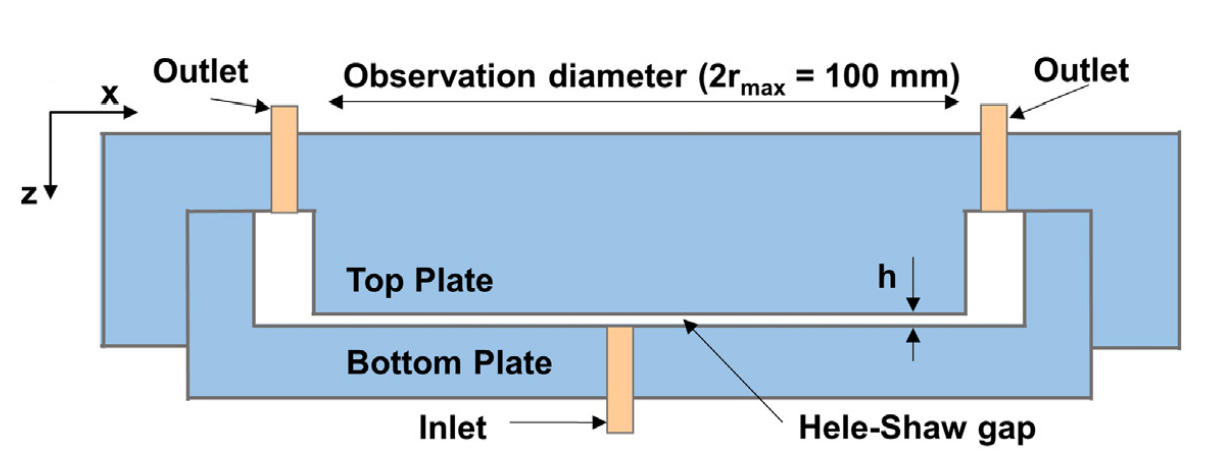
\includegraphics[scale=0.4]{experimental_setup}
	\caption{Experimental setup used to generate existing experimental data used for validation \cite{stergiou2022effects}}
	\label{fig: experiment}
\end{figure}
The Hele-Shaw gap is formed by two plates sitting on top of each other. The inlet is located on the bottom at the centreline of the reactor. The outlets are located at the top with an empty space that is needed to get no influence from outlet on the flow field within the gap. The gap height $h$ used for the experiments was 0.2mm. The experiment is observed by a camera from the top throughout the whole run. The gained images are further analysed by image processing. The images are captured as greyscale images. The gained values are correlated to concentration values using the known values for the input's concentrations. Based on the gained product concentration values the reaction front's front and back positions are calculated using a threshold operation. The position of the fronts maximum is computed by detecting the position of the maximum grey value within the image. In addition to the front's positions the total amount of product formed is calculated. This is done by integrating the concentration values over the whole domain and gap height.

%To make experiments more easily comparable with each other the formed product values (in mol) are non-dimensionalized. To achieve this the values are divided by $c_{max} \cdot V_{reactor}$. The variable $c_{max}$ is the maximum value of the product's concentration during one experimental run and $V_{reactor}$ is the reactor's volume. The product of these two values refers to the fully mixed case as it gives in indication of the maximum amount of product possible than can be created. The volume injected is equivalent to the time elapsed in seconds. These two values can be converted using the flow rate. NC is the non-dimensional product formed for each time step.


\subsection{Model Results}
\label{sec: model res}
The model results are created at each interval defined by the user as described in \autoref{sec: setup}. The gained tables do have a format similar to \autoref{tab: model_csv}. The values for each cell are stored in one of the table rows. The cells are distinguishable by their x and y coordinate.

\begin{table} [htb]
	\centering
	\caption{Simulation output table example}
	\small
	\begin{tabular}{ cccccc }
		\hline
		nodenumber & x-coordinate & y-coordinate & ... & concentration-fluid\_c & ... \\
		\hline
		1 & 1.206592076E-06 & 5.0E-04 & ... & 5.681614735E-11 & ...\\
		... & ... & ... & ... & ... & ... \\
		100 & 1.382432295E-06 & 5.12E-04 & ... & 3.607185187E-17 & ... \\
		... & ... & ... & ... & ... & ... \\
		\hline
		\label{tab: model_csv}
	\end{tabular}
\end{table}

All values needed are accessible with these tables but for further analysis the values need to be converted into a field similar to the created mesh shown in \autoref{fig:ansys_meshing} during model setup. An example of such a resulting field is shown in \autoref{fig: field_example}.
\begin{figure}[htbp]
	\centering
	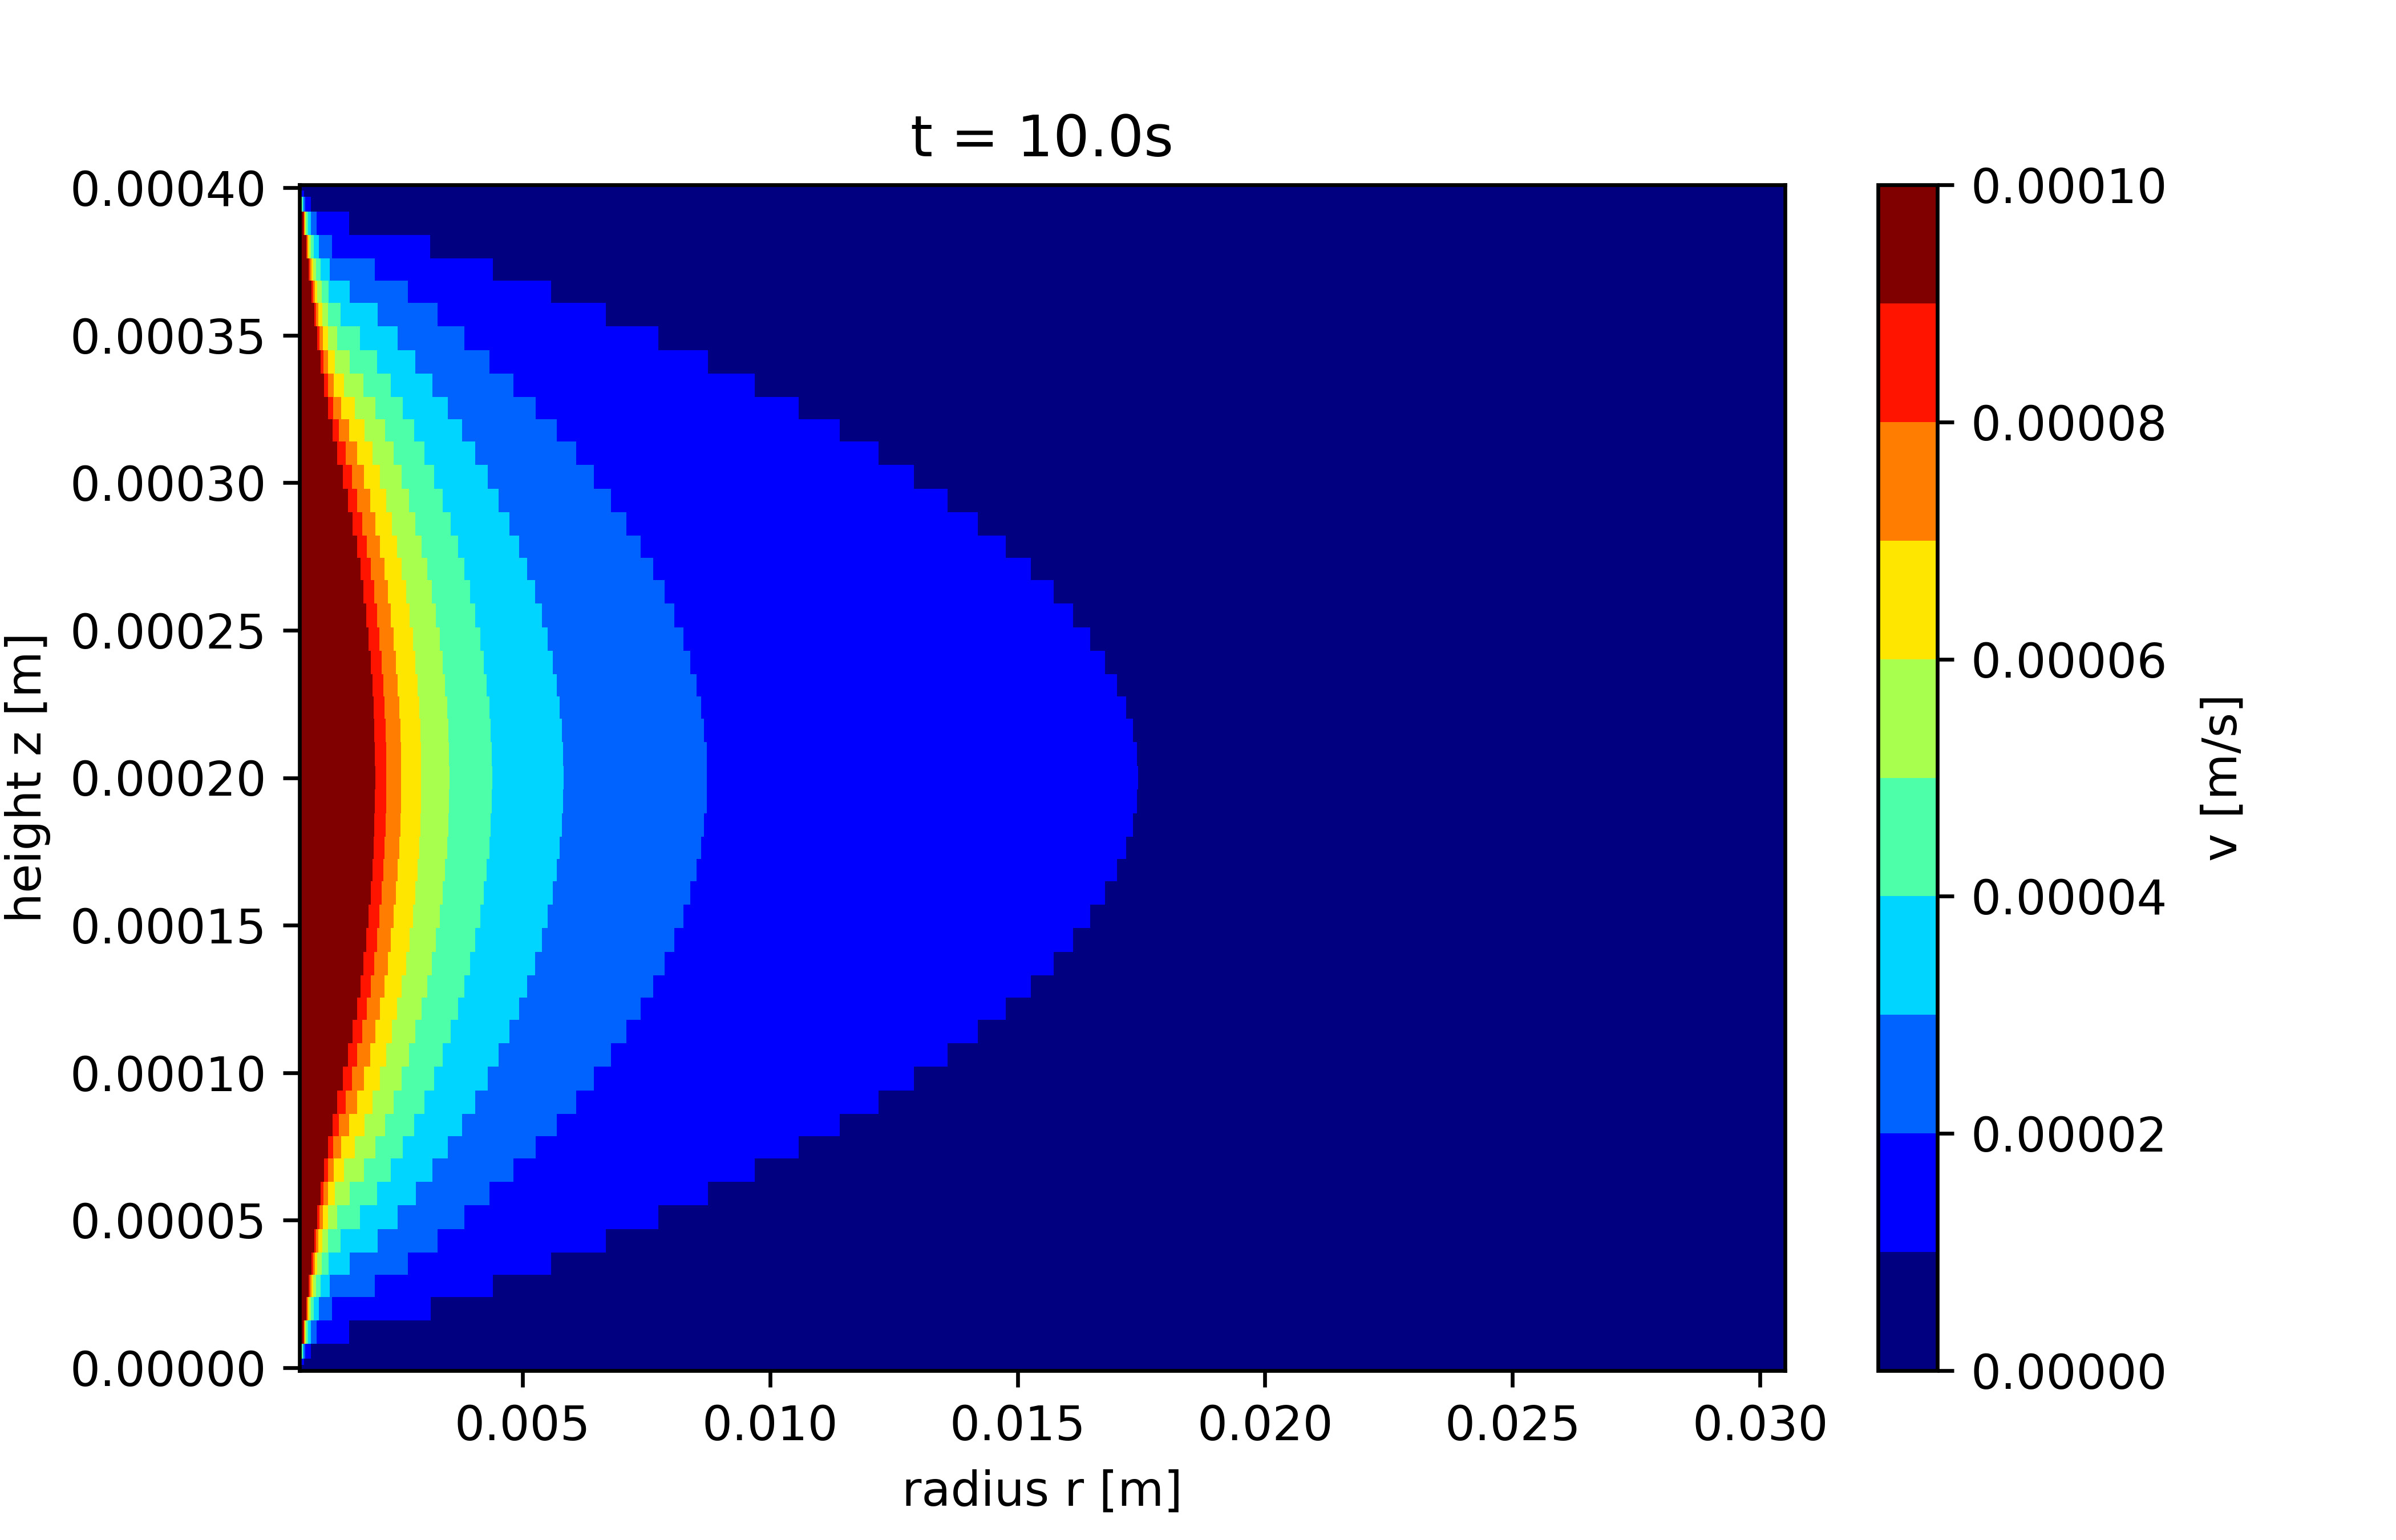
\includegraphics[width=0.9\textwidth]{field_h4r3_P931E2_S120E4_velocity-magnitude}
	\caption{example field representation (velocity field) of model results}
	\label{fig: field_example}
\end{figure}
These fields can be created for all exported variables. Within the example shown the field is created for the velocity magnitude but the variable of most interest is the product concentration. A field example for this variable is shown in \autoref{fig: c_plot_prod_example} for 3 different time steps.
\begin{figure}[htb]
	\centering
	\subfloat[\centering gap averaged concentrations]{{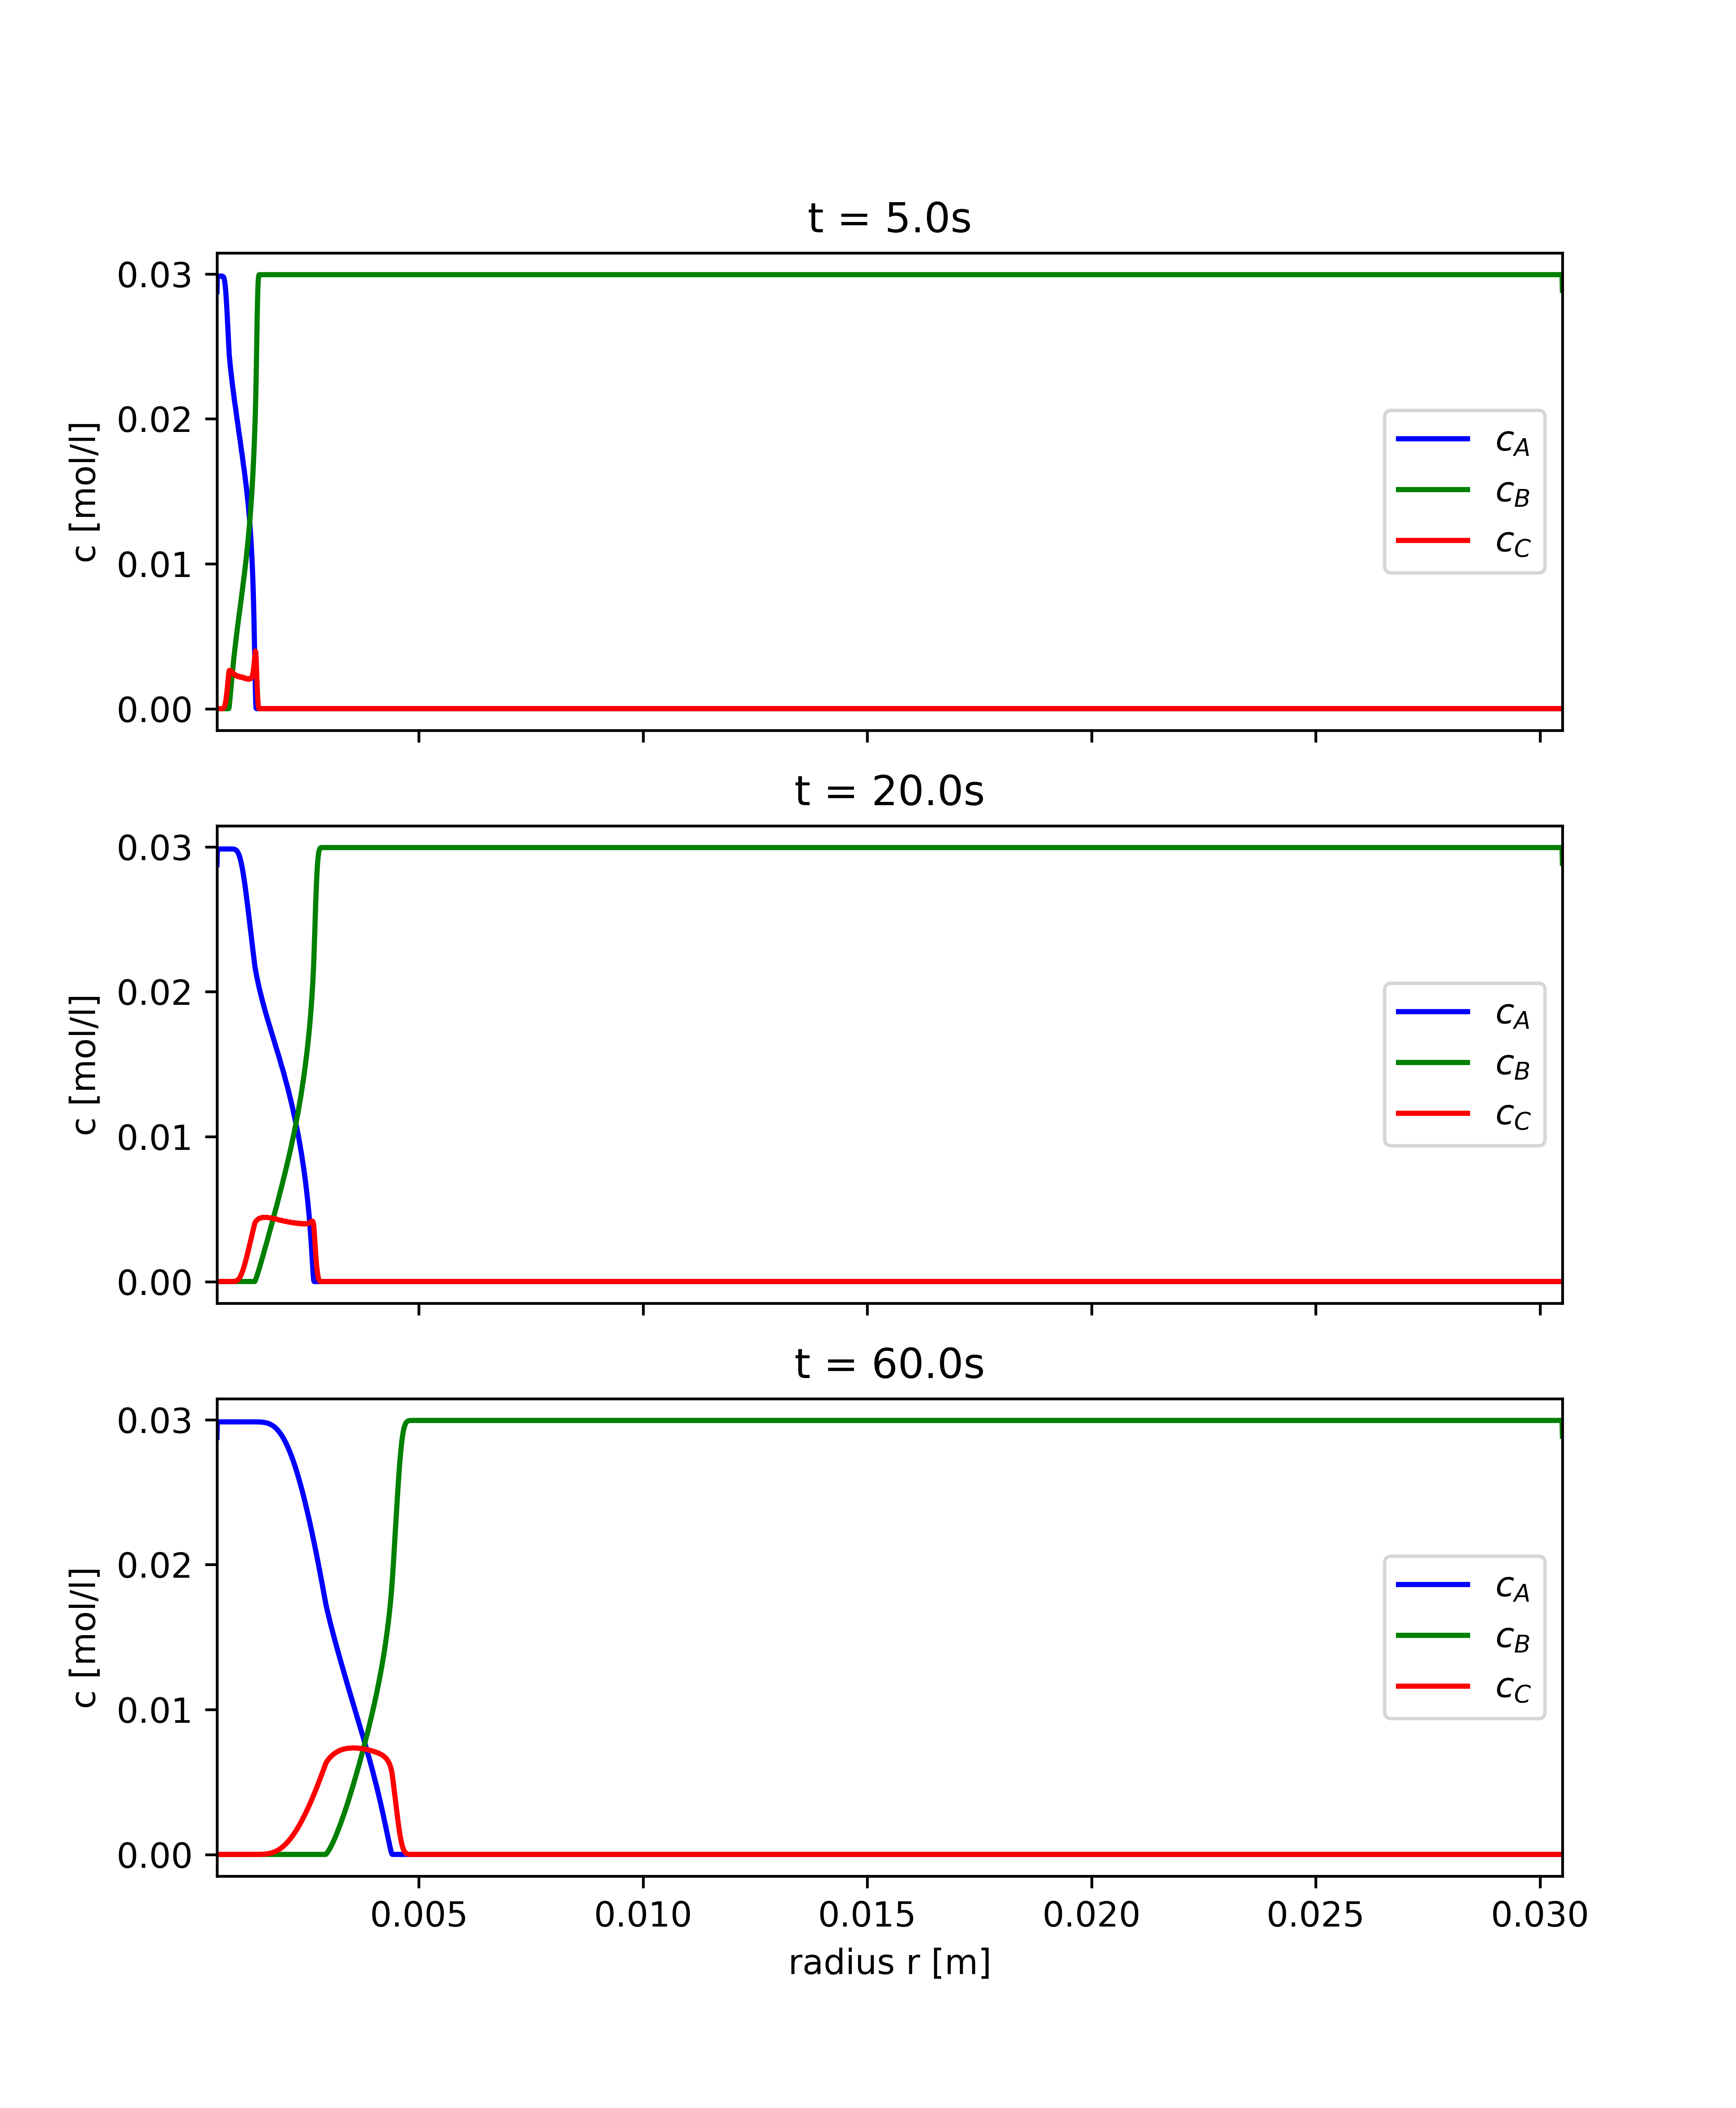
\includegraphics[angle=0, scale=0.41]{plot_h4r3_P931E2_S120E4_concentration-fluid_a_concentration-fluid_b_concentration-fluid_c} }}%
	\qquad
	\subfloat[\centering product concentration fields]{{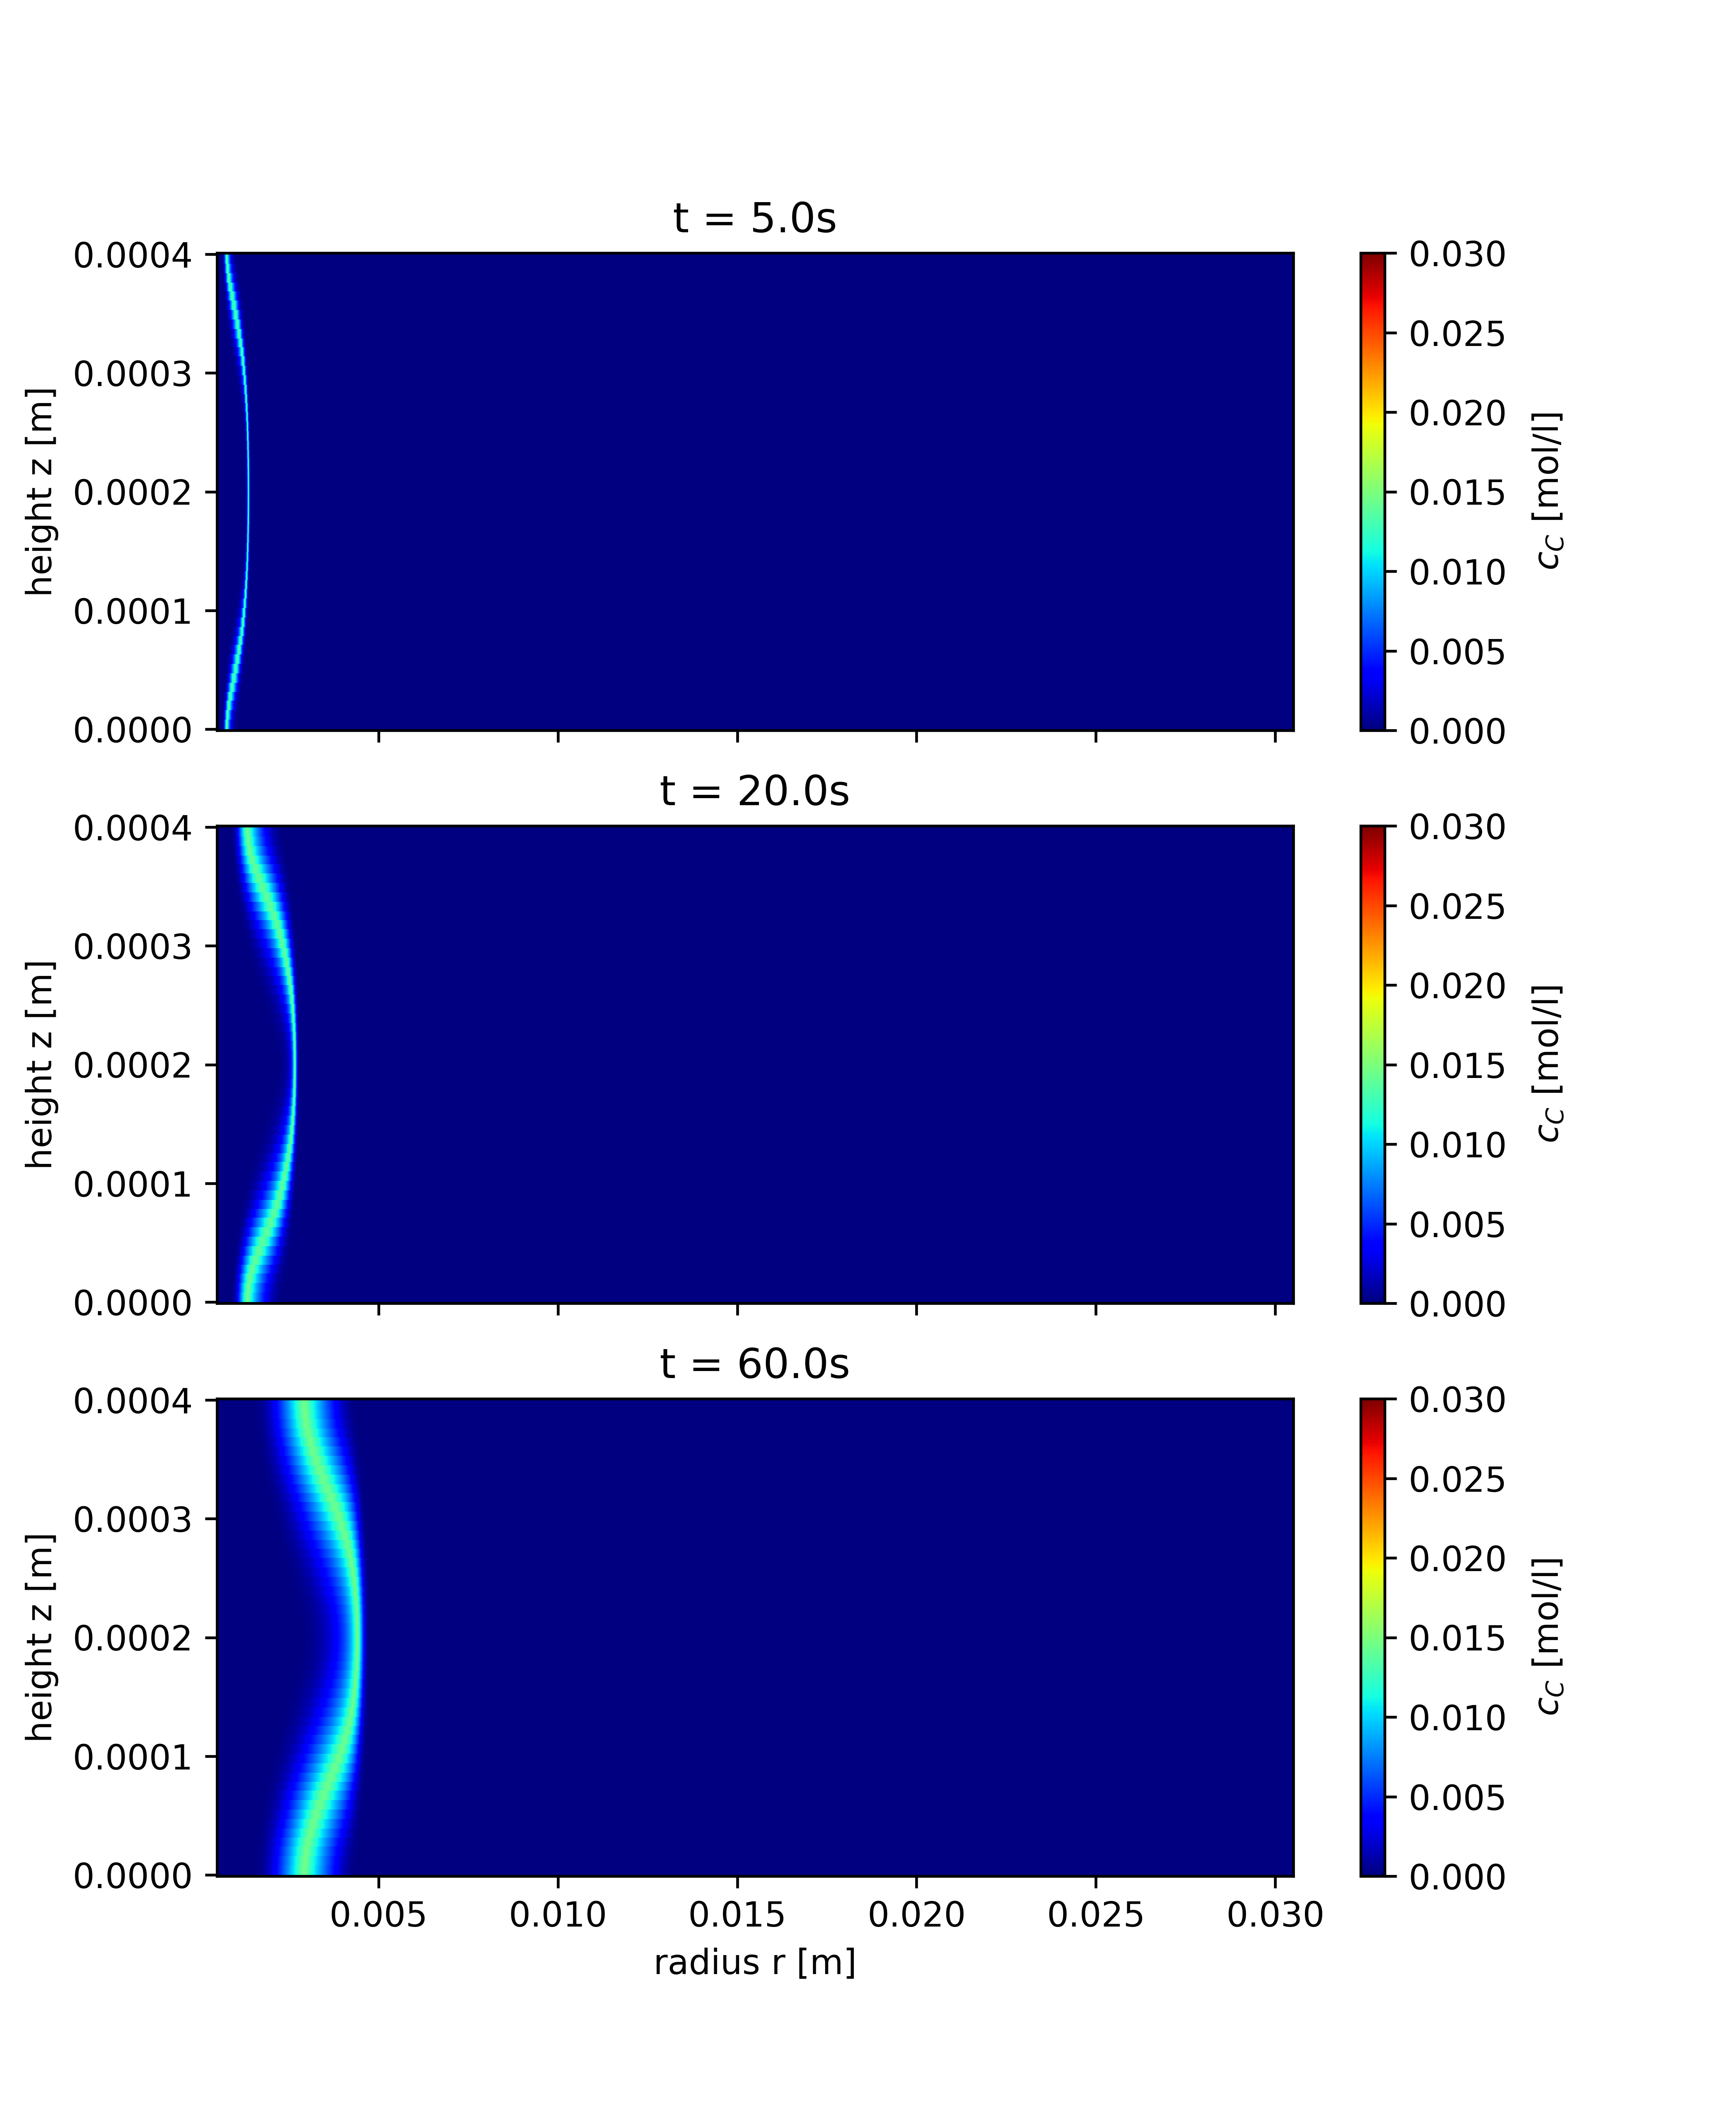
\includegraphics[angle=0, scale=0.41]{field_h4r3_P931E2_S120E4_concentration-fluid_c} }}%
	\caption{field and averaged concentration example}%
	\label{fig: c_plot_prod_example}%
\end{figure}
With these fields the products concentration can be averaged over the whole gap height. This step is done to get a comparable post-processing step to the image processing done on the experimental data sets. The resulting plots from the previous example can also bee seen in \autoref{fig: c_plot_prod_example}.

With the fields and the gap averaged concentration values computed the parameters of interest can be calculated. How that is done is explained within the following sections.

\subsubsection{Front Positions}

The front's maximum position is gained by storing the radial positions of the product's maxima within the concentration plots. The front's front position is calculated by using the the position furthest away from the center at half the maximums value. The positions gained are shown for one time step in \autoref{fig: pos_examp} as an example.

\begin{figure}[htb]
	\centering
	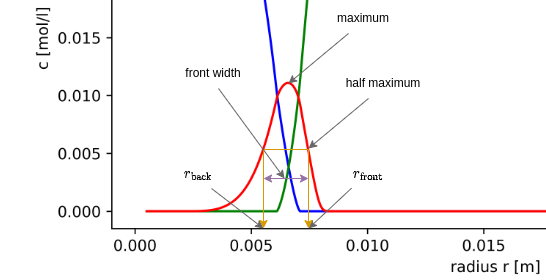
\includegraphics[scale=0.5]{positions_examp}
	\caption{front position procedure schematic}
	\label{fig: pos_examp}
\end{figure}

\subsubsection{Front Width}

For calculating the front widths the fronts front and back positions are needed. The front position is already gained and the back position is computed using the same approach. Instead of taking for furthest position away from the center the closest one to the inlet is taken to get the back position. The difference between these two radial positions is the front's width at the time. The width calculated is visualized in \autoref{fig: pos_examp}. The approach for calculating the width is also known as \textbf{F}ull \textbf{W}idth at \textbf{H}alf \textbf{M}aximum or FWHM in short.

To gain some more insights a second width is computed. The second width is calculated at the middle of the gap height using the same procedure. The width at half of the reactors gap height also described as \textbf{F}ull \textbf{W}idth at \textbf{H}alf \textbf{M}aximum at \textbf{H}alf \textbf{G}ap \textbf{H}eight is called FWHMHGH in short. Instead of taking the gap averaged values, the values used here are the field values themselves at half the gap height. This width that is only calculated using one height position behaves similar to a 1D case with a decaying velocity towards high radial values.

The difference between the two calculated widths is that the FWHM is influenced by the concentration values in the whole gap, compared to the FWHMHGH that is only influenced by the concentration values along the radial position at a constant height. The FWMHGH is expected to only grow, whereas the FWHM could grow and shrink dependent on the fronts curvature.

\subsubsection{Product Formed}

Since the cell volume and the product concentration for each cell are accessible from the results exported, the total amount of product formed can be calculated by multiplying these two columns with each other. \texttt{ANSYS FLUENT} computes it's values for one radiant for a 2D axisymmetric case. To gain the amount of product within the whole reactor the values have to be multiplied by $2 \pi$. This procedure can be described by \autoref{eqn: tot_prod}. $ n_{C, total} $ is the total amount of product produced, $n_{cells}$ is the amount of cells in the mesh, $ V_i $ is the volume of one cell and $c_{i, C}$ the product's concentration within that cell $i$.

\begin{equation}
	n_{C, total} = 2 \pi \cdot \sum_{i=0}^{n_{cells}} \left[ V_i \cdot c_{i, C} \right]
	\label{eqn: tot_prod} 
\end{equation}

\subsection{Comparison}

For comparison the position of the product's maximum is used. From \autoref{fig: comp_maxis} it can be seen that the model and experiment perform similar over the whole time range with a small deviation at early time steps. These differences might come from slightly different flow conditions or some mixing due to gravitational influences. All in all the model provides valid results as shown in the graph.
\begin{figure}[htbp]
	\centering
	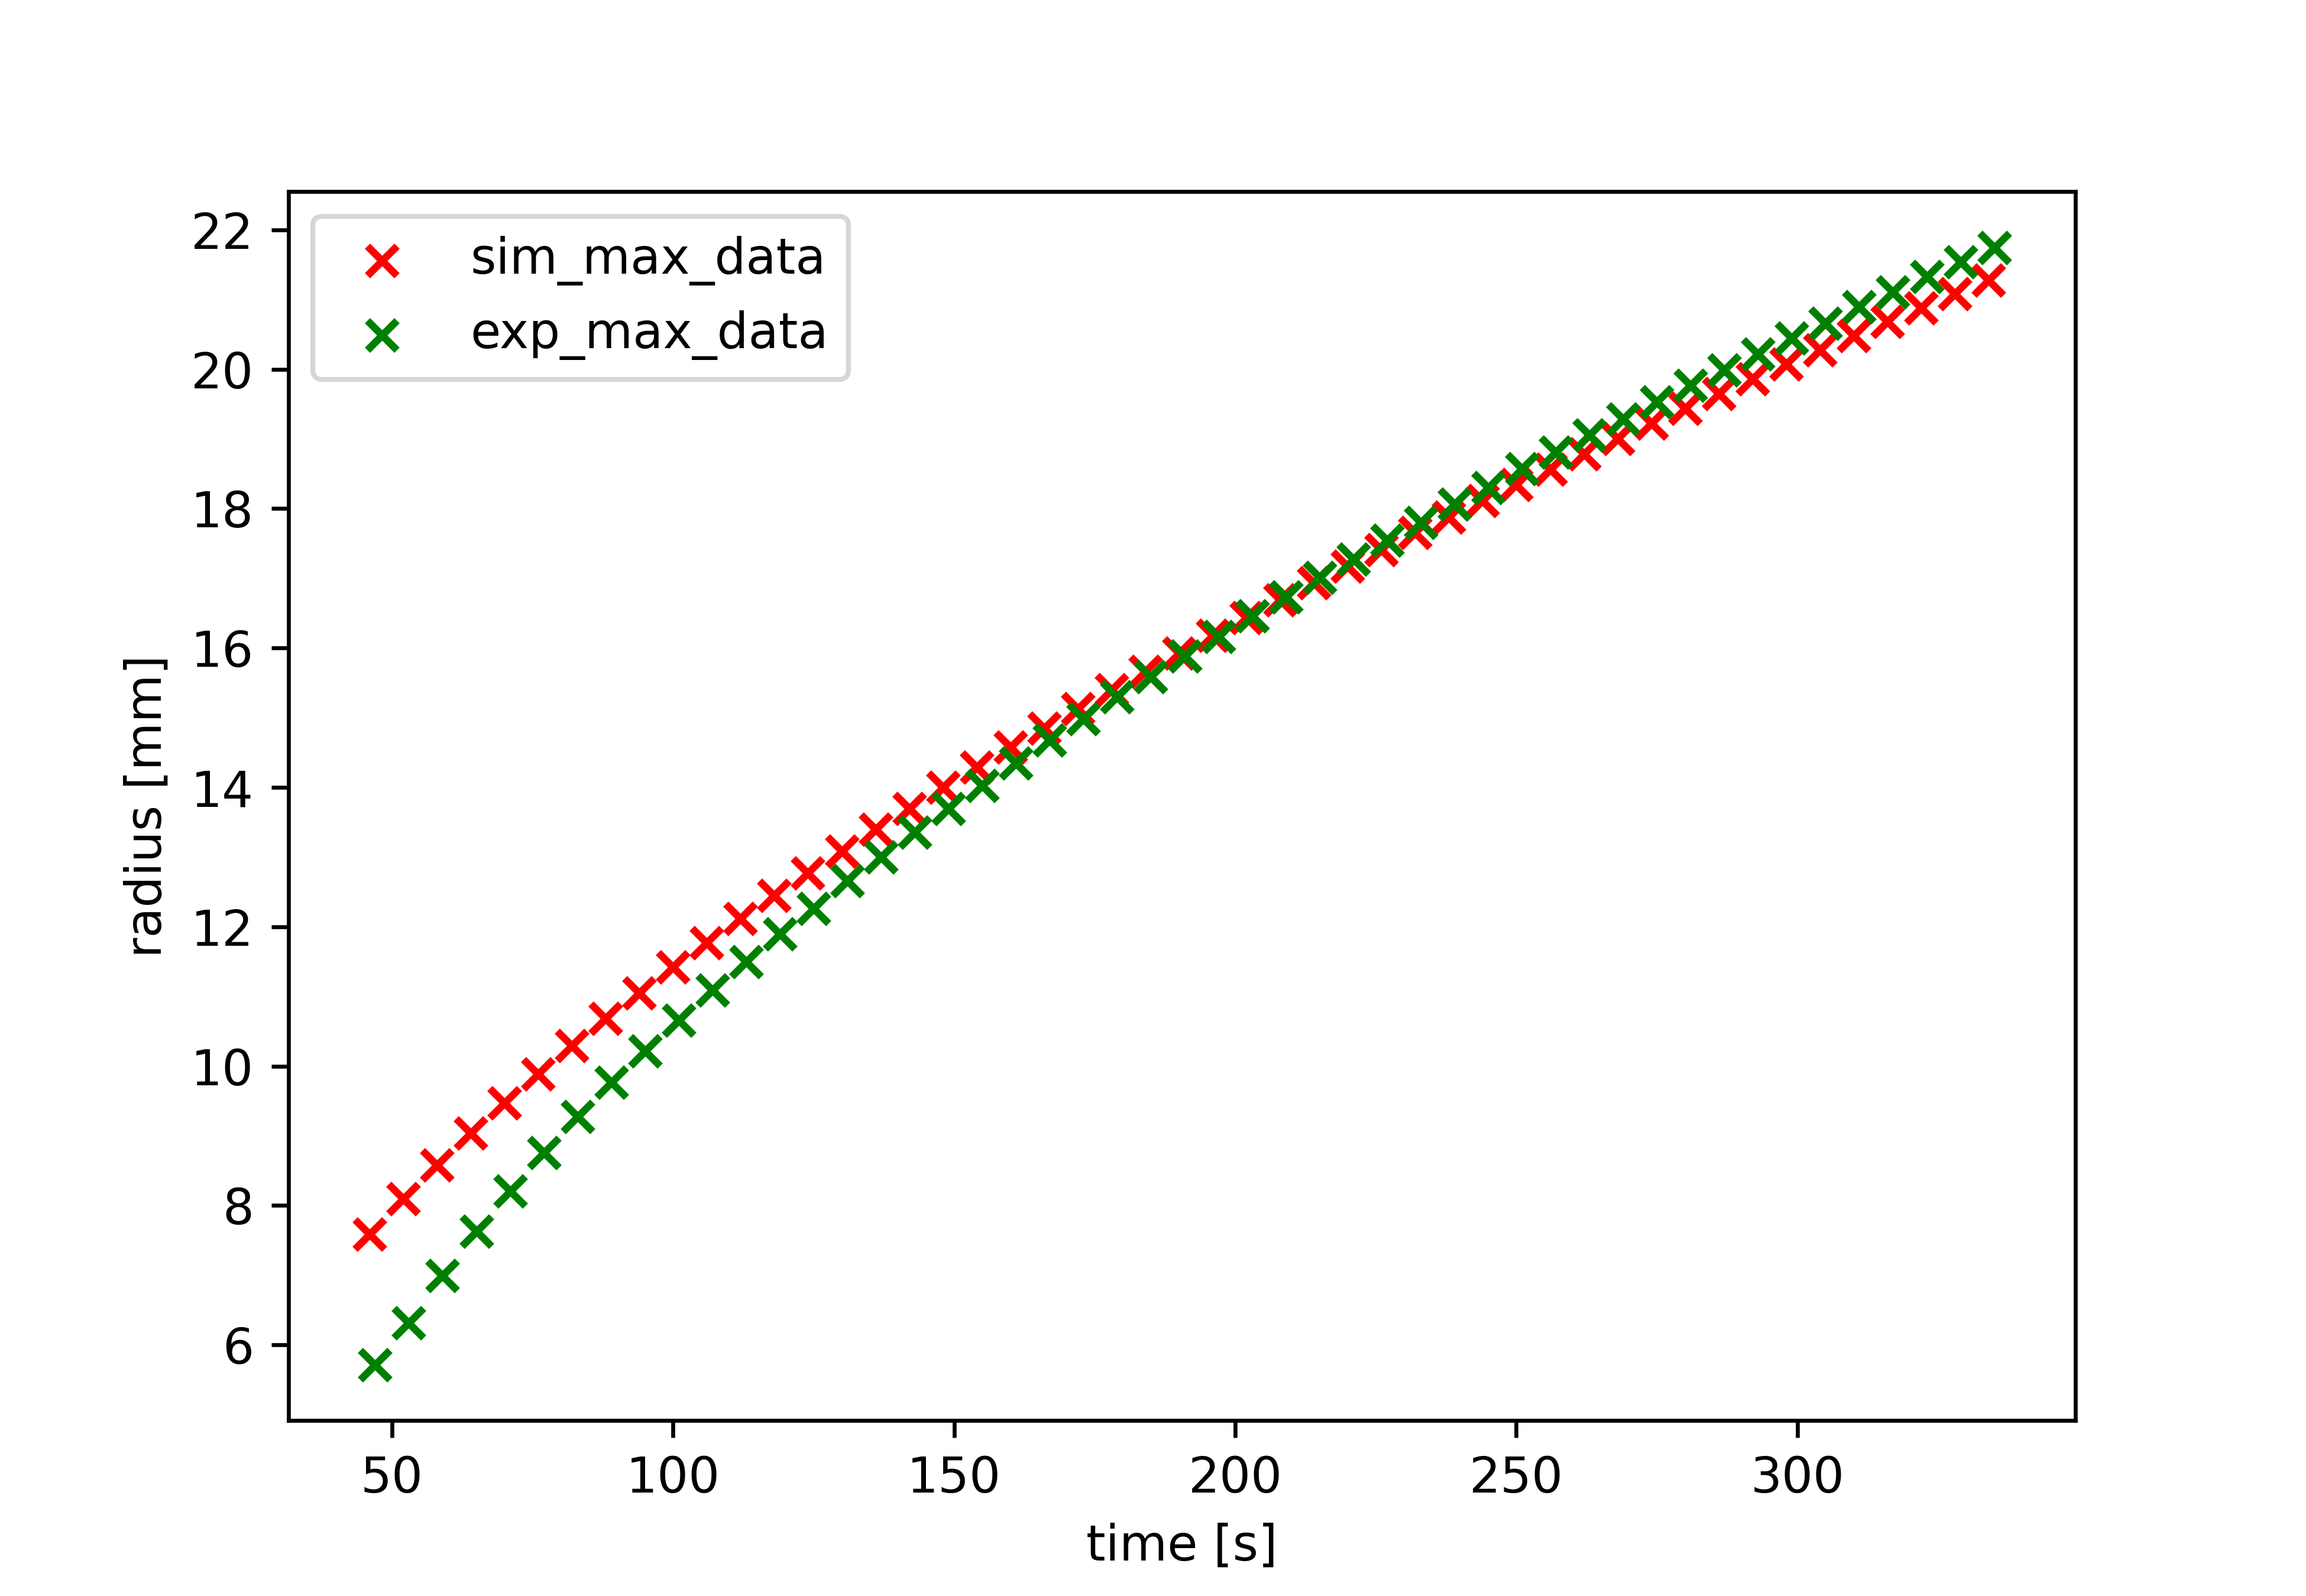
\includegraphics[width=\textwidth]{front_exp}
	\caption{comparison of the experimental and model maxima positions}
	\label{fig: comp_maxis}
\end{figure}


\end{document}